%======================================================
% CHAPTER IV: SWD - SOFTWARE DESIGN DESCRIPTION
%======================================================
\chapter{SWD -- MÔ TẢ THIẾT KẾ PHẦN MỀM}

\section{Tổng quan Thiết kế}

Chương này trình bày \textbf{Mô tả Thiết kế Phần mềm (Software Design Description -- SWD)} cho hệ thống Chatbot RAG. Tài liệu này mô tả chi tiết kiến trúc hệ thống, thiết kế cơ sở dữ liệu và thiết kế các thành phần phần mềm thông qua các biểu đồ UML bao gồm: Use Case chi tiết, Class Diagram, State Machine Diagram, Flowchart và Activity Diagram.

%------------------------------------------------------
\section{Thiết kế Kiến trúc Hệ thống (System Architecture)}
%------------------------------------------------------

\subsection{Kiến trúc Tổng thể}

Hệ thống được xây dựng theo mô hình \textbf{Client-Server} kết hợp với \textbf{AI Pipeline} chuyên biệt cho RAG:

\begin{figure}[H]
  \centering
  
\includegraphics[width=0.95\textwidth]{images/context.png}
  \caption{Kiến trúc tổng thể hệ thống Chatbot RAG}
  \label{fig:architecture}
\end{figure}

Kiến trúc hệ thống được phân tách thành 5 lớp rõ ràng:
\begin{enumerate}[itemsep=3pt]
  \item \textbf{Presentation Layer (Frontend ReactJS):} Giao diện người dùng, xử lý tương tác và render dữ liệu.
  \item \textbf{API Gateway Layer (FastAPI Router):} Tiếp nhận, xác thực và định tuyến request.
  \item \textbf{Business Logic Layer (Services):} Điều phối RAG Pipeline, Benchmark Module, Document Service.
  \item \textbf{Data Access Layer:} Giao tiếp với ChromaDB (Vector) và MySQL (Quan hệ).
  \item \textbf{External Services Layer:} Gemini API, BAAI/bge-m3 Embedding.
\end{enumerate}

\subsection{Package Diagram}

\begin{figure}[H]
  \centering
  \begin{tikzpicture}[
    pkg/.style={rectangle, draw=blue!60, fill=blue!5, rounded corners=3pt,
                minimum width=3.2cm, minimum height=1.2cm, align=center, font=\small},
    ext/.style={rectangle, draw=orange!70, fill=orange!5, rounded corners=3pt,
                minimum width=3cm, minimum height=1cm, align=center, font=\small, dashed},
    db/.style={cylinder, draw=green!60!black, fill=green!5,
                minimum width=2.5cm, minimum height=1cm, align=center, font=\small,
                shape border rotate=90, aspect=0.25},
    arrow/.style={-Stealth, thick},
    node distance=1.2cm
  ]
    % Frontend
    \node[pkg] (frontend) {\textbf{Frontend}\\\texttt{ReactJS}};

    % Backend packages
    \node[pkg, right=2.5cm of frontend] (router) {\textbf{API Router}\\\texttt{FastAPI}};
    \node[pkg, above right=1cm and 1.5cm of router] (rag) {\textbf{RAG Service}\\\texttt{Python}};
    \node[pkg, right=1.5cm of router] (doc) {\textbf{Document\\ Service}};
    \node[pkg, below right=1cm and 1.5cm of router] (bench) {\textbf{Benchmark\\ Module}};

    % Databases
    \node[db, right=2.5cm of doc] (chroma) {ChromaDB};
    \node[db, right=2.5cm of bench] (mysql) {MySQL};

    % External
    \node[ext, above=1.5cm of chroma] (gemini) {Gemini API\\(LLM + Embed)};
    \node[ext, right=1.5cm of chroma] (bge) {BAAI/bge-m3\\(Local Embed)};

    % Arrows
    \draw[arrow] (frontend) -- (router);
    \draw[arrow] (router) -- (rag);
    \draw[arrow] (router) -- (doc);
    \draw[arrow] (router) -- (bench);
    \draw[arrow] (rag) -- (chroma);
    \draw[arrow] (doc) -- (chroma);
    \draw[arrow] (doc) -- (mysql);
    \draw[arrow] (bench) -- (mysql);
    \draw[arrow] (rag) -- (gemini);
    \draw[arrow] (rag) -- (bge);
  \end{tikzpicture}
  \caption{Package Diagram hệ thống}
  \label{fig:package-diagram}
\end{figure}

%------------------------------------------------------
\section{Thiết kế Cơ sở Dữ liệu (Database Design)}
%------------------------------------------------------

\subsection{Entity Relationship Diagram (ERD)}

\begin{figure}[H]
  \centering
  
\includegraphics[width=\textwidth]{images/erd.png}
  \caption{Sơ đồ thực thể quan hệ (ERD) của hệ thống}
  \label{fig:erd}
\end{figure}

\subsection{Mô tả Các Bảng Dữ liệu Chính}

\begin{table}[H]
  \centering
  \caption{Mô tả bảng \texttt{users}}
  \label{tab:db-users}
  \renewcommand{\arraystretch}{1.4}
  \begin{tabularx}{\textwidth}{|l|l|l|X|}
    \hline
    \rowcolor{blue!10}
    \textbf{Cột} & \textbf{Kiểu dữ liệu} & \textbf{Ràng buộc} & \textbf{Mô tả} \\
    \hline
    id & INT & PK, AUTO\_INCREMENT & Khóa chính. \\
    username & VARCHAR(100) & NOT NULL, UNIQUE & Tên đăng nhập. \\
    email & VARCHAR(255) & NOT NULL, UNIQUE & Địa chỉ email. \\
    password\_hash & VARCHAR(255) & NOT NULL & Mật khẩu đã băm. \\
    role & ENUM & NOT NULL & Vai trò: student / admin. \\
    created\_at & DATETIME & DEFAULT NOW() & Ngày tạo tài khoản. \\
    \hline
  \end{tabularx}
\end{table}

\begin{table}[H]
  \centering
  \caption{Mô tả bảng \texttt{documents}}
  \label{tab:db-documents}
  \renewcommand{\arraystretch}{1.4}
  \begin{tabularx}{\textwidth}{|l|l|l|X|}
    \hline
    \rowcolor{blue!10}
    \textbf{Cột} & \textbf{Kiểu dữ liệu} & \textbf{Ràng buộc} & \textbf{Mô tả} \\
    \hline
    id & INT & PK, AUTO\_INCREMENT & Khóa chính. \\
    file\_name & VARCHAR(255) & NOT NULL & Tên file gốc. \\
    subject & VARCHAR(100) & & Môn học liên quan. \\
    total\_chunks & INT & DEFAULT 0 & Số lượng chunk sau Ingestion. \\
    status & ENUM & NOT NULL & Trạng thái: processing / ready / error. \\
    uploaded\_by & INT & FK → users.id & ID người tải lên. \\
    uploaded\_at & DATETIME & DEFAULT NOW() & Thời điểm tải lên. \\
    chroma\_collection & VARCHAR(100) & & Tên collection trong ChromaDB. \\
    \hline
  \end{tabularx}
\end{table}

\begin{table}[H]
  \centering
  \caption{Mô tả bảng \texttt{conversations} và \texttt{messages}}
  \label{tab:db-chat}
  \renewcommand{\arraystretch}{1.4}
  \begin{tabularx}{\textwidth}{|l|l|l|X|}
    \hline
    \rowcolor{blue!10}
    \textbf{Cột} & \textbf{Kiểu dữ liệu} & \textbf{Ràng buộc} & \textbf{Mô tả} \\
    \hline
    \multicolumn{4}{|c|}{\cellcolor{gray!20} \textbf{Bảng: conversations}} \\
    \hline
    id & INT & PK & Khóa chính phiên trò chuyện. \\
    user\_id & INT & FK → users.id & Người dùng sở hữu phiên. \\
    created\_at & DATETIME & DEFAULT NOW() & Thời điểm tạo phiên. \\
    \hline
    \multicolumn{4}{|c|}{\cellcolor{gray!20} \textbf{Bảng: messages}} \\
    \hline
    id & INT & PK & Khóa chính tin nhắn. \\
    conversation\_id & INT & FK → conversations.id & Phiên trò chuyện. \\
    role & ENUM & NOT NULL & user / assistant. \\
    content & TEXT & NOT NULL & Nội dung tin nhắn. \\
    sources & JSON & & Danh sách nguồn trích dẫn. \\
    latency\_ms & INT & & Thời gian phản hồi (ms). \\
    created\_at & DATETIME & DEFAULT NOW() & Thời điểm gửi tin nhắn. \\
    \hline
  \end{tabularx}
\end{table}

\begin{table}[H]
  \centering
  \caption{Mô tả bảng \texttt{experiments} và \texttt{evaluations}}
  \label{tab:db-benchmark}
  \renewcommand{\arraystretch}{1.4}
  \begin{tabularx}{\textwidth}{|l|l|l|X|}
    \hline
    \rowcolor{blue!10}
    \textbf{Cột} & \textbf{Kiểu dữ liệu} & \textbf{Ràng buộc} & \textbf{Mô tả} \\
    \hline
    \multicolumn{4}{|c|}{\cellcolor{gray!20} \textbf{Bảng: experiments}} \\
    \hline
    id & INT & PK & Khóa chính kịch bản. \\
    name & VARCHAR(200) & NOT NULL & Tên kịch bản Benchmark. \\
    chunking\_strategy & VARCHAR(50) & NOT NULL & Chiến lược Chunking sử dụng. \\
    embedding\_model & VARCHAR(100) & NOT NULL & Mô hình Embedding sử dụng. \\
    llm\_model & VARCHAR(100) & NOT NULL & Mô hình LLM sử dụng. \\
    avg\_accuracy & FLOAT & & Điểm Accuracy trung bình. \\
    avg\_faithfulness & FLOAT & & Điểm Faithfulness trung bình. \\
    avg\_relevancy & FLOAT & & Điểm Relevancy trung bình. \\
    avg\_latency\_ms & FLOAT & & Latency trung bình (ms). \\
    created\_at & DATETIME & DEFAULT NOW() & Thời điểm chạy. \\
    \hline
    \multicolumn{4}{|c|}{\cellcolor{gray!20} \textbf{Bảng: evaluations}} \\
    \hline
    id & INT & PK & Khóa chính đánh giá. \\
    experiment\_id & INT & FK → experiments.id & Kịch bản tương ứng. \\
    question & TEXT & NOT NULL & Câu hỏi trong test set. \\
    ground\_truth & TEXT & NOT NULL & Đáp án chuẩn. \\
    generated\_answer & TEXT & NOT NULL & Câu trả lời AI sinh ra. \\
    accuracy & FLOAT & & Điểm Accuracy từng câu. \\
    faithfulness & FLOAT & & Điểm Faithfulness từng câu. \\
    relevancy & FLOAT & & Điểm Relevancy từng câu. \\
    latency\_ms & INT & & Thời gian xử lý (ms). \\
    \hline
  \end{tabularx}
\end{table}

%------------------------------------------------------
\section{Thiết kế Chi tiết (Detailed Design)}
%------------------------------------------------------

\subsection{Biểu đồ Lớp (Class Diagram)}

\begin{figure}[H]
  \centering
  
\includegraphics[width=\textwidth]{images/class_diagram.png}
  \caption{Biểu đồ Lớp (Class Diagram) của hệ thống}
  \label{fig:class-diagram}
\end{figure}

Hệ thống được thiết kế xung quanh các lớp chính:

\begin{table}[H]
  \centering
  \caption{Mô tả các lớp trong Class Diagram}
  \label{tab:classes}
  \renewcommand{\arraystretch}{1.4}
  \begin{tabularx}{\textwidth}{|l|X|}
    \hline
    \rowcolor{blue!10}
    \textbf{Tên Lớp} & \textbf{Trách nhiệm} \\
    \hline
    \texttt{User} (abstract) & Lớp trừu tượng chung cho người dùng, định nghĩa các thuộc tính cơ bản (id, username, email, role). \\
    \hline
    \texttt{SinhVien} & Kế thừa User; cung cấp phương thức \texttt{send\_question()}, \texttt{get\_history()}, \texttt{configure\_rag()}. \\
    \hline
    \texttt{QuanTriVien} & Kế thừa User; bổ sung \texttt{upload\_document()}, \texttt{delete\_document()}, \texttt{run\_benchmark()}. \\
    \hline
    \texttt{HeThongChatbot} & Lớp điều phối trung tâm (Facade). Nhận \texttt{CauHoi}, điều phối RAG Pipeline, trả về \texttt{CauTraLoi}. \\
    \hline
    \texttt{TaiLieuMonHoc} & Đóng gói tài liệu: đọc file, chunking, gọi Embedding, lưu ChromaDB. \\
    \hline
    \texttt{MoHinhAI} (interface) & Interface chung cho LLM và Embedding Model. Phương thức: \texttt{generate(prompt)}, \texttt{embed(text)}. \\
    \hline
    \texttt{GeminiAdapter} & Triển khai \texttt{MoHinhAI} cho Gemini API. \\
    \hline
    \texttt{BGEAdapter} & Triển khai \texttt{MoHinhAI} cho BAAI/bge-m3 cục bộ. \\
    \hline
    \texttt{ChromaDBRepository} & Lớp truy xuất dữ liệu Vector: \texttt{insert()}, \texttt{search(vector, top\_k)}, \texttt{delete()}. \\
    \hline
    \texttt{BenchmarkService} & Điều phối kịch bản Benchmark: nạp test set, vòng lặp đánh giá, tính RAGAS metrics. \\
    \hline
    \texttt{BaoCaoPhanTich} & Tổng hợp số liệu Benchmark, tạo dữ liệu cho Radar Chart và bảng xếp hạng. \\
    \hline
  \end{tabularx}
\end{table}

%----------------------------------------------
\subsection{Biểu đồ Trạng thái (State Machine Diagram)}
%----------------------------------------------

\subsubsection{State Machine: Vòng đời Tài liệu (Document Lifecycle)}

\begin{figure}[H]
  \centering
  \begin{tikzpicture}[
    state/.style={rectangle, draw=blue!60, fill=blue!8, rounded corners=6pt,
                  minimum width=3.2cm, minimum height=1cm, align=center, font=\small\bfseries},
    initstate/.style={circle, draw=black, fill=black, minimum size=12pt},
    finalstate/.style={circle, draw=black, fill=black, minimum size=12pt,
                        double, double distance=2pt},
    arrow/.style={-Stealth, thick, blue!70},
    label/.style={font=\scriptsize, text=gray!80!black},
    node distance=2.5cm
  ]
    \node[initstate] (init) {};
    \node[state, right=1.5cm of init] (idle) {Chờ tải lên\\(Idle)};
    \node[state, right=of idle] (uploading) {Đang tải lên\\(Uploading)};
    \node[state, right=of uploading] (processing) {Đang xử lý\\(Processing)};
    \node[state, below=of processing] (ready) {Sẵn sàng\\(Ready)};
    \node[state, below=of uploading] (error) {Lỗi\\(Error)};
    \node[finalstate, left=1.5cm of error] (final) {};

    \draw[arrow] (init) -- (idle);
    \draw[arrow] (idle) -- node[above, label]{Chọn file} (uploading);
    \draw[arrow] (uploading) -- node[above, label]{Upload OK} (processing);
    \draw[arrow] (uploading) -- node[right, label]{Upload fail} (error);
    \draw[arrow] (processing) -- node[right, label]{Ingestion OK} (ready);
    \draw[arrow] (processing) -- node[above, label]{Parse fail} (error);
    \draw[arrow] (ready) to[bend left=50] node[right, label]{Xóa tài liệu} (final);
    \draw[arrow] (error) -- node[above, label]{Xóa} (final);
    \draw[arrow] (error) to[bend right=30] node[right, label]{Thử lại} (uploading);
  \end{tikzpicture}
  \caption{State Machine Diagram: Vòng đời Tài liệu (Document Lifecycle)}
  \label{fig:state-document}
\end{figure}

\textbf{Mô tả các trạng thái:}
\begin{table}[H]
  \centering
  \caption{Mô tả trạng thái tài liệu}
  \label{tab:doc-states}
  \renewcommand{\arraystretch}{1.4}
  \begin{tabularx}{\textwidth}{|l|X|X|}
    \hline
    \rowcolor{blue!10}
    \textbf{Trạng thái} & \textbf{Điều kiện vào} & \textbf{Hành động} \\
    \hline
    Idle & Khởi tạo hệ thống & Hiển thị nút Upload. \\
    \hline
    Uploading & Admin chọn file và nhấn Upload & Gửi file lên server, hiển thị progress bar. \\
    \hline
    Processing & Upload thành công & Chạy Ingestion Pipeline: extract → chunk → embed → store. \\
    \hline
    Ready & Ingestion Pipeline hoàn tất & Tài liệu sẵn sàng cho chat RAG. \\
    \hline
    Error & Upload hoặc Parsing thất bại & Ghi log lỗi, hiển thị thông báo, cho phép thử lại. \\
    \hline
  \end{tabularx}
\end{table}

\subsubsection{State Machine: Vòng đời Phiên Hội thoại (Chat Session)}

\begin{figure}[H]
  \centering
  \begin{tikzpicture}[
    state/.style={rectangle, draw=green!60!black, fill=green!5, rounded corners=6pt,
                  minimum width=3cm, minimum height=1cm, align=center, font=\small\bfseries},
    initstate/.style={circle, draw=black, fill=black, minimum size=12pt},
    finalstate/.style={circle, draw=black, fill=black, minimum size=12pt,
                        double, double distance=2pt},
    arrow/.style={-Stealth, thick, green!60!black},
    label/.style={font=\scriptsize, text=gray!80!black},
    node distance=2.2cm
  ]
    \node[initstate] (init) {};
    \node[state, right=1.5cm of init] (idle) {Chờ nhập\\câu hỏi};
    \node[state, right=of idle] (sending) {Đang gửi\\câu hỏi};
    \node[state, right=of sending] (retrieving) {Truy xuất\\ChromaDB};
    \node[state, below=of retrieving] (generating) {Sinh câu\\trả lời (LLM)};
    \node[state, left=of generating] (displaying) {Hiển thị\\kết quả};
    \node[finalstate, left=1.5cm of displaying] (final) {};

    \draw[arrow] (init) -- (idle);
    \draw[arrow] (idle) -- node[above, label]{Submit} (sending);
    \draw[arrow] (sending) -- node[above, label]{Embed OK} (retrieving);
    \draw[arrow] (retrieving) -- node[right, label]{Top-K retrieved} (generating);
    \draw[arrow] (generating) -- node[below, label]{Response ready} (displaying);
    \draw[arrow] (displaying) to[bend right=15] node[above, label]{Câu hỏi tiếp} (idle);
    \draw[arrow] (displaying) -- node[above, label]{Kết thúc} (final);
  \end{tikzpicture}
  \caption{State Machine Diagram: Vòng đời Phiên Hội thoại (Chat Session)}
  \label{fig:state-chat}
\end{figure}

%----------------------------------------------
\subsection{Biểu đồ Luồng (Flowchart)}
%----------------------------------------------

\subsubsection{Flowchart: RAG Pipeline (Luồng Hỏi đáp)}

\begin{figure}[H]
  \centering
  \begin{tikzpicture}[
    block/.style={rectangle, draw=blue!60, fill=blue!5, rounded corners=4pt,
                  minimum width=5cm, minimum height=0.9cm, align=center, font=\small},
    decision/.style={diamond, draw=orange!70, fill=orange!5,
                     minimum width=4cm, minimum height=1cm, align=center,
                     font=\small, aspect=2},
    start/.style={rounded rectangle, draw=green!60!black, fill=green!8,
                  minimum width=4cm, minimum height=0.8cm, align=center, font=\small\bfseries},
    end/.style={rounded rectangle, draw=red!60, fill=red!5,
                minimum width=4cm, minimum height=0.8cm, align=center, font=\small\bfseries},
    arrow/.style={-Stealth, thick},
    node distance=0.9cm
  ]
    \node[start] (start) {BẮT ĐẦU: Sinh viên gửi câu hỏi};
    \node[block, below=of start] (embed) {Mã hóa câu hỏi thành Vector Embedding};
    \node[block, below=of embed] (search) {Tìm kiếm Top-K chunks trong ChromaDB (Cosine Similarity)};
    \node[decision, below=of search] (found) {Tìm thấy\\kết quả?};
    \node[block, below=of found] (build) {Xây dựng Prompt Template với Top-K ngữ cảnh};
    \node[block, below=of build] (llm) {Gọi LLM API (Gemini 2.5 Flash)};
    \node[block, below=of llm] (response) {Nhận câu trả lời từ LLM};
    \node[block, below=of response] (save) {Lưu lịch sử vào MySQL, gán nguồn trích dẫn};
    \node[end, below=of save] (end) {Trả về kết quả cho Frontend};
    \node[block, right=3cm of found] (nofound) {Trả về thông báo:\\``Không tìm thấy thông tin''};

    \draw[arrow] (start) -- (embed);
    \draw[arrow] (embed) -- (search);
    \draw[arrow] (search) -- (found);
    \draw[arrow] (found) -- node[left]{\small Có} (build);
    \draw[arrow] (found) -- node[above]{\small Không} (nofound);
    \draw[arrow] (build) -- (llm);
    \draw[arrow] (llm) -- (response);
    \draw[arrow] (response) -- (save);
    \draw[arrow] (save) -- (end);
    \draw[arrow] (nofound) |- (end);
  \end{tikzpicture}
  \caption{Flowchart: RAG Pipeline -- Luồng xử lý câu hỏi hỏi đáp}
  \label{fig:flowchart-rag}
\end{figure}

\subsubsection{Flowchart: Ingestion Pipeline (Luồng Xử lý Tài liệu)}

\begin{figure}[H]
  \centering
  \begin{tikzpicture}[
    block/.style={rectangle, draw=purple!60, fill=purple!5, rounded corners=4pt,
                  minimum width=5.5cm, minimum height=0.9cm, align=center, font=\small},
    decision/.style={diamond, draw=orange!70, fill=orange!5,
                     minimum width=4.5cm, minimum height=1cm, align=center,
                     font=\small, aspect=2.2},
    start/.style={rounded rectangle, draw=green!60!black, fill=green!8,
                  minimum width=4.5cm, minimum height=0.8cm, align=center, font=\small\bfseries},
    end/.style={rounded rectangle, draw=red!60, fill=red!5,
                minimum width=4.5cm, minimum height=0.8cm, align=center, font=\small\bfseries},
    arrow/.style={-Stealth, thick},
    node distance=0.9cm
  ]
    \node[start] (start) {BẮT ĐẦU: Admin tải lên file PDF/DOCX};
    \node[decision, below=of start] (valid) {File hợp lệ?\\(định dạng, kích thước)};
    \node[block, below=of valid] (extract) {Trích xuất văn bản thô (PyPDF / pdfplumber)};
    \node[block, below=of extract] (clean) {Làm sạch văn bản (loại ký tự nhiễu, chuẩn hóa)};
    \node[block, below=of clean] (chunk) {Phân mảnh (Chunking) theo chiến lược được chọn};
    \node[block, below=of chunk] (embed) {Tạo Vector Embedding cho từng chunk};
    \node[block, below=of embed] (store) {Lưu Vector + metadata vào ChromaDB};
    \node[block, below=of store] (meta) {Cập nhật metadata tài liệu vào MySQL (status = Ready)};
    \node[end, below=of meta] (end) {KẾT THÚC: Tài liệu sẵn sàng};
    \node[block, right=3.5cm of valid] (error) {Cập nhật status = Error,\\ thông báo Admin};

    \draw[arrow] (start) -- (valid);
    \draw[arrow] (valid) -- node[left]{\small Hợp lệ} (extract);
    \draw[arrow] (valid) -- node[above]{\small Không hợp lệ} (error);
    \draw[arrow] (extract) -- (clean);
    \draw[arrow] (clean) -- (chunk);
    \draw[arrow] (chunk) -- (embed);
    \draw[arrow] (embed) -- (store);
    \draw[arrow] (store) -- (meta);
    \draw[arrow] (meta) -- (end);
    \draw[arrow] (error) |- (end);
  \end{tikzpicture}
  \caption{Flowchart: Ingestion Pipeline -- Luồng xử lý tài liệu}
  \label{fig:flowchart-ingestion}
\end{figure}

\subsubsection{Flowchart: Benchmark Pipeline}

\begin{figure}[H]
  \centering
  \begin{tikzpicture}[
    block/.style={rectangle, draw=teal!60, fill=teal!5, rounded corners=4pt,
                  minimum width=5.5cm, minimum height=0.9cm, align=center, font=\small},
    decision/.style={diamond, draw=orange!70, fill=orange!5,
                     minimum width=4cm, minimum height=1cm, align=center,
                     font=\small, aspect=2},
    start/.style={rounded rectangle, draw=green!60!black, fill=green!8,
                  minimum width=5cm, minimum height=0.8cm, align=center, font=\small\bfseries},
    end/.style={rounded rectangle, draw=red!60, fill=red!5,
                minimum width=5cm, minimum height=0.8cm, align=center, font=\small\bfseries},
    arrow/.style={-Stealth, thick},
    node distance=0.9cm
  ]
    \node[start] (start) {BẮT ĐẦU: Admin cấu hình và chạy Benchmark};
    \node[block, below=of start] (load) {Nạp Test Dataset (50 câu hỏi + Ground Truth)};
    \node[block, below=of load] (init) {Khởi tạo cấu hình (Chunking + Embedding + LLM)};
    \node[block, below=of init] (loop) {Lấy câu hỏi tiếp theo từ Test Dataset};
    \node[block, below=of loop] (run) {Chạy toàn bộ RAG Pipeline cho câu hỏi};
    \node[block, below=of run] (score) {Tính điểm RAGAS: Accuracy, Faithfulness, Relevancy, Latency};
    \node[decision, below=of score] (more) {Còn câu hỏi?};
    \node[block, below=of more] (avg) {Tính trung bình toàn bộ chỉ số};
    \node[block, below=of avg] (save) {Lưu kết quả vào MySQL (experiments, evaluations)};
    \node[end, below=of save] (end) {KẾT THÚC: Cập nhật Dashboard};

    \draw[arrow] (start) -- (load);
    \draw[arrow] (load) -- (init);
    \draw[arrow] (init) -- (loop);
    \draw[arrow] (loop) -- (run);
    \draw[arrow] (run) -- (score);
    \draw[arrow] (score) -- (more);
    \draw[arrow] (more) to[bend left=50] node[right]{\small Còn} (loop);
    \draw[arrow] (more) -- node[left]{\small Hết} (avg);
    \draw[arrow] (avg) -- (save);
    \draw[arrow] (save) -- (end);
  \end{tikzpicture}
  \caption{Flowchart: Benchmark Pipeline}
  \label{fig:flowchart-benchmark}
\end{figure}

%----------------------------------------------
\subsection{Biểu đồ Hoạt động (Activity Diagram)}
%----------------------------------------------

\subsubsection{Activity Diagram: Tương tác Chat giữa Sinh viên và Hệ thống}

\begin{figure}[H]
  \centering
  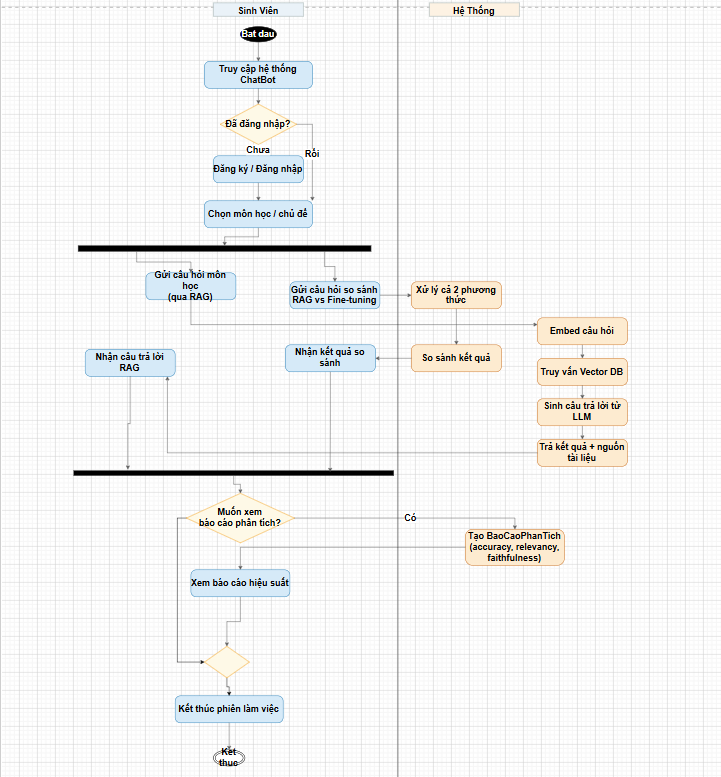
\includegraphics[width=\textwidth]{images/active-diagram_sinhvien.png}
  \caption{Activity Diagram: Tương tác Chat giữa Sinh viên và Hệ thống}
  \label{fig:activity-chat}
\end{figure}

\subsubsection{Activity Diagram: Quản trị viên Upload và Quản lý Tài liệu}

\begin{figure}[H]
  \centering
  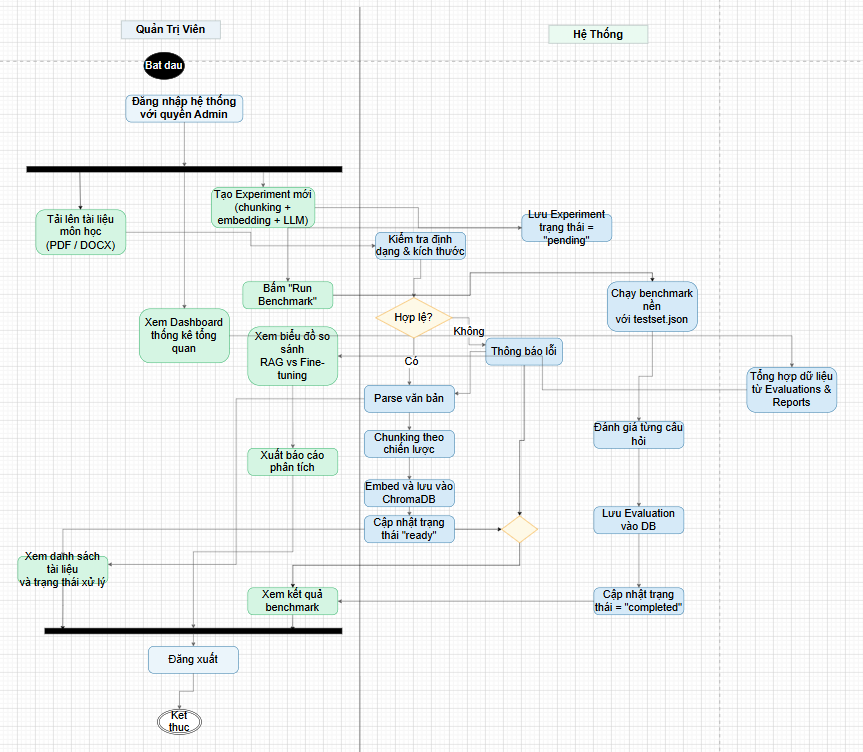
\includegraphics[width=\textwidth]{images/SRS/active_quantrivien.png}
  \caption{Activity Diagram: Quản trị viên Upload và Quản lý Tài liệu}
  \label{fig:activity-admin}
\end{figure}

\subsubsection{Activity Diagram: Quy trình Benchmark}

\begin{figure}[H]
  \centering
  \begin{tikzpicture}[
    act/.style={rectangle, draw=teal!60, fill=teal!5, rounded corners=4pt,
                minimum width=5cm, minimum height=0.85cm, align=center, font=\small},
    decision/.style={diamond, draw=orange!70, fill=orange!10,
                     minimum width=3.5cm, align=center, font=\small, aspect=2},
    initstate/.style={circle, draw=black, fill=black, minimum size=10pt},
    finalstate/.style={circle, draw=black, fill=black, minimum size=12pt,
                        double, double distance=2pt},
    fork/.style={rectangle, draw=black, fill=black, minimum width=4cm, minimum height=4pt},
    arrow/.style={-Stealth, thick},
    label/.style={font=\scriptsize},
    node distance=0.9cm
  ]
    \node[initstate] (init) {};
    \node[act, below=0.5cm of init] (config) {Admin cấu hình kịch bản Benchmark};
    \node[act, below=of config] (load) {Nạp Test Dataset (50 câu hỏi)};
    \node[act, below=of load] (setenv) {Khởi tạo môi trường (Chunking + Embedding)};
    \node[decision, below=of setenv] (loop) {Còn câu hỏi\\ trong dataset?};
    \node[act, below=of loop] (run) {Chạy RAG Pipeline cho câu hỏi hiện tại};
    \node[act, below=of run] (eval) {Đánh giá RAGAS: Acc, Faith, Rel, Lat};
    \node[act, below=of eval] (store) {Lưu kết quả từng câu vào evaluations};
    \node[act, right=3cm of loop] (agg) {Tổng hợp điểm trung bình};
    \node[act, below=of agg] (save) {Lưu vào experiments table};
    \node[act, below=of save] (dashboard) {Cập nhật Dashboard (Radar Chart)};
    \node[finalstate, below=of dashboard] (final) {};

    \draw[arrow] (init) -- (config);
    \draw[arrow] (config) -- (load);
    \draw[arrow] (load) -- (setenv);
    \draw[arrow] (setenv) -- (loop);
    \draw[arrow] (loop) -- node[left]{\small Còn} (run);
    \draw[arrow] (run) -- (eval);
    \draw[arrow] (eval) -- (store);
    \draw[arrow] (store) to[bend right=50] node[right]{\small Câu tiếp} (loop);
    \draw[arrow] (loop) -- node[above]{\small Hết} (agg);
    \draw[arrow] (agg) -- (save);
    \draw[arrow] (save) -- (dashboard);
    \draw[arrow] (dashboard) -- (final);
  \end{tikzpicture}
  \caption{Activity Diagram: Quy trình Benchmark đánh giá RAG}
  \label{fig:activity-benchmark}
\end{figure}

%----------------------------------------------
\subsection{Biểu đồ Use Case Chi tiết (Detailed Use Case)}
%----------------------------------------------

\subsubsection{UC-01: Đặt câu hỏi Chat RAG}

\begin{table}[H]
  \centering
  \caption{Đặc tả Use Case UC-01: Chat RAG}
  \label{tab:uc01}
  \renewcommand{\arraystretch}{1.5}
  \begin{tabularx}{\textwidth}{|l|X|}
    \hline
    \rowcolor{blue!10}
    \textbf{Mục} & \textbf{Nội dung} \\
    \hline
    Use Case ID & UC-01 \\
    \hline
    Tên & Chat RAG -- Hỏi đáp bằng AI từ tài liệu \\
    \hline
    Actor & Sinh viên (Primary), LLM (Secondary), ChromaDB (Secondary) \\
    \hline
    Pre-condition & Hệ thống có ít nhất 1 tài liệu ở trạng thái ``Ready'' trong ChromaDB. \\
    \hline
    Trigger & Sinh viên nhập câu hỏi và nhấn ``Gửi''. \\
    \hline
    Main Flow &
      1. Sinh viên nhập câu hỏi vào Chat Sandbox.\newline
      2. Hệ thống nhận request và mã hóa câu hỏi thành Vector.\newline
      3. ChromaDB tìm Top-K chunks tương đồng nhất.\newline
      4. Backend xây dựng Prompt với ngữ cảnh từ các chunks.\newline
      5. Backend gọi Gemini API, nhận câu trả lời.\newline
      6. Hệ thống trả về câu trả lời + danh sách nguồn trích dẫn.\newline
      7. Frontend hiển thị và lưu lịch sử. \\
    \hline
    Alternative Flow & Nếu ChromaDB không tìm thấy kết quả → Hệ thống trả về MSG-03. \\
    \hline
    Post-condition & Câu hỏi và câu trả lời được lưu vào bảng \texttt{messages}. \\
    \hline
  \end{tabularx}
\end{table}

\subsubsection{UC-08: Chạy Benchmark}

\begin{table}[H]
  \centering
  \caption{Đặc tả Use Case UC-08: Benchmark}
  \label{tab:uc08}
  \renewcommand{\arraystretch}{1.5}
  \begin{tabularx}{\textwidth}{|l|X|}
    \hline
    \rowcolor{blue!10}
    \textbf{Mục} & \textbf{Nội dung} \\
    \hline
    Use Case ID & UC-08 \\
    \hline
    Tên & Chạy Benchmark đánh giá cấu hình RAG \\
    \hline
    Actor & Quản trị viên (Primary) \\
    \hline
    Pre-condition & Admin đã đăng nhập; Test Dataset tồn tại; ít nhất 1 tài liệu trong ChromaDB. \\
    \hline
    Trigger & Admin cấu hình kịch bản và nhấn ``Chạy Benchmark''. \\
    \hline
    Main Flow &
      1. Admin chọn cấu hình: Chunking Strategy + Embedding Model.\newline
      2. Hệ thống nạp Test Dataset (50 câu hỏi + Ground Truth).\newline
      3. Với mỗi câu hỏi: chạy RAG Pipeline và tính điểm RAGAS.\newline
      4. Hệ thống tính điểm trung bình toàn bộ kịch bản.\newline
      5. Lưu kết quả vào \texttt{experiments} và \texttt{evaluations}.\newline
      6. Cập nhật Dashboard với kết quả mới. \\
    \hline
    Alternative Flow & Nếu LLM API lỗi → Ghi log lỗi và thông báo Admin. \\
    \hline
    Post-condition & Kết quả Benchmark được lưu và hiển thị trên Dashboard. \\
    \hline
  \end{tabularx}
\end{table}

\section{Thiết kế Giao diện Người dùng (UI Design)}

\subsection{Giao diện Trang chủ}

\begin{figure}[H]
  \centering
  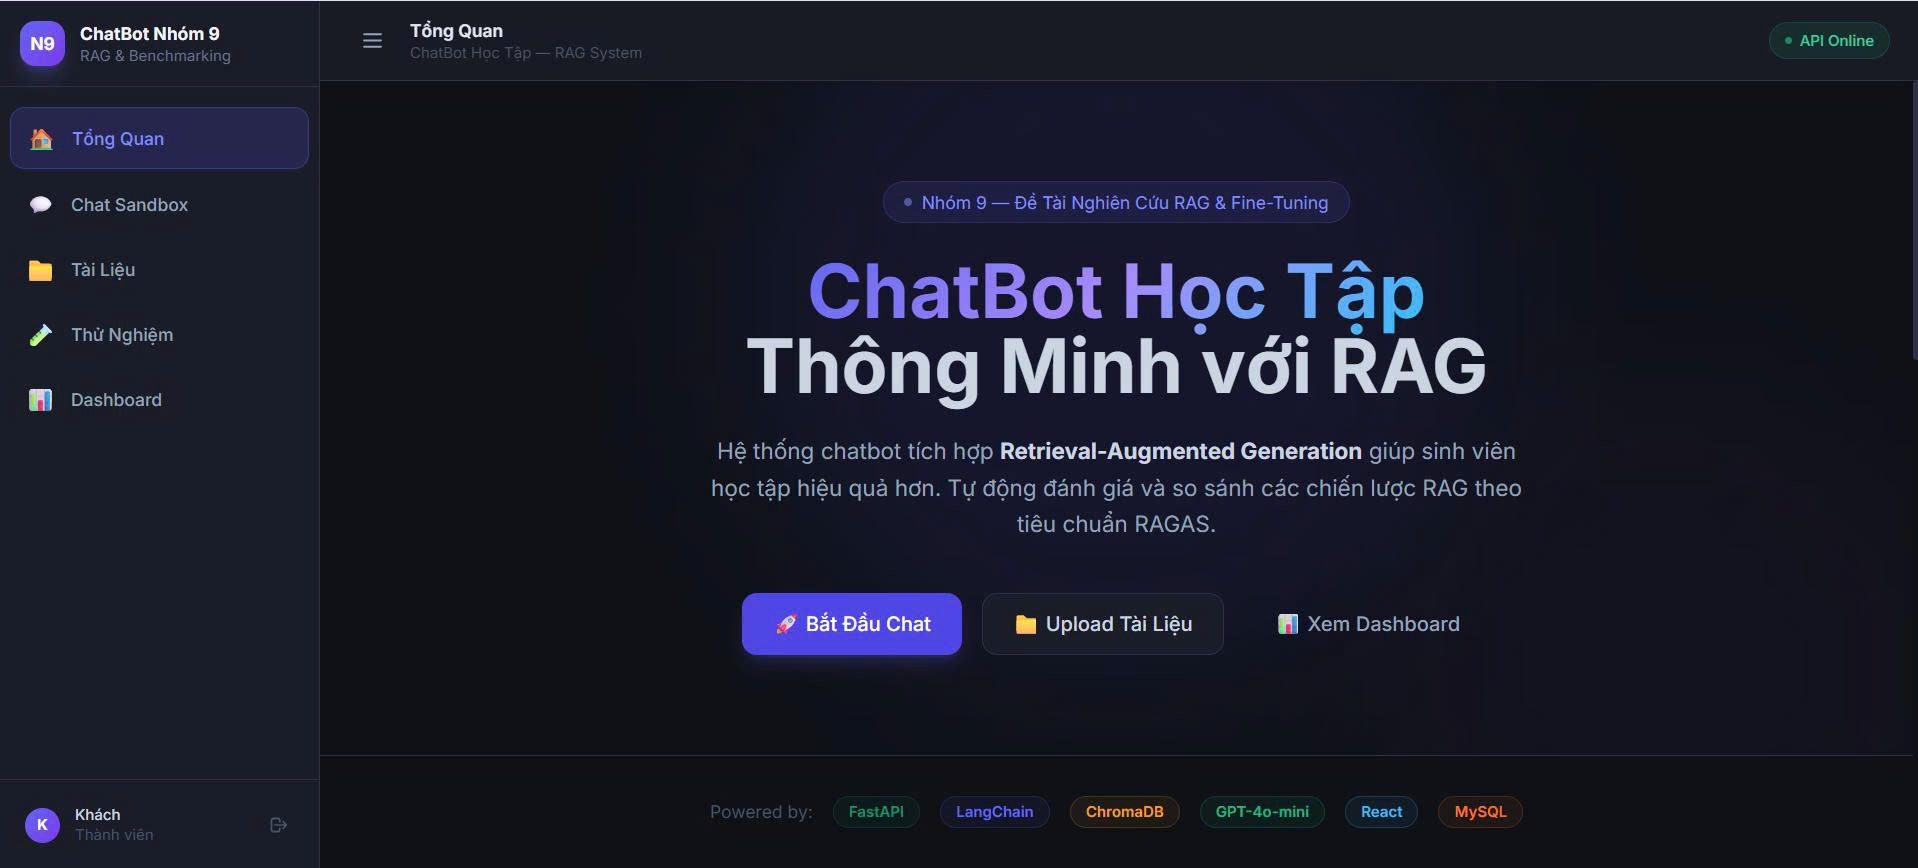
\includegraphics[width=\textwidth]{images/ui_home.png}
  \caption{Giao diện Trang chủ hệ thống}
  \label{fig:ui-home}
\end{figure}

\subsection{Giao diện Chat Sandbox}

\begin{figure}[H]
  \centering
  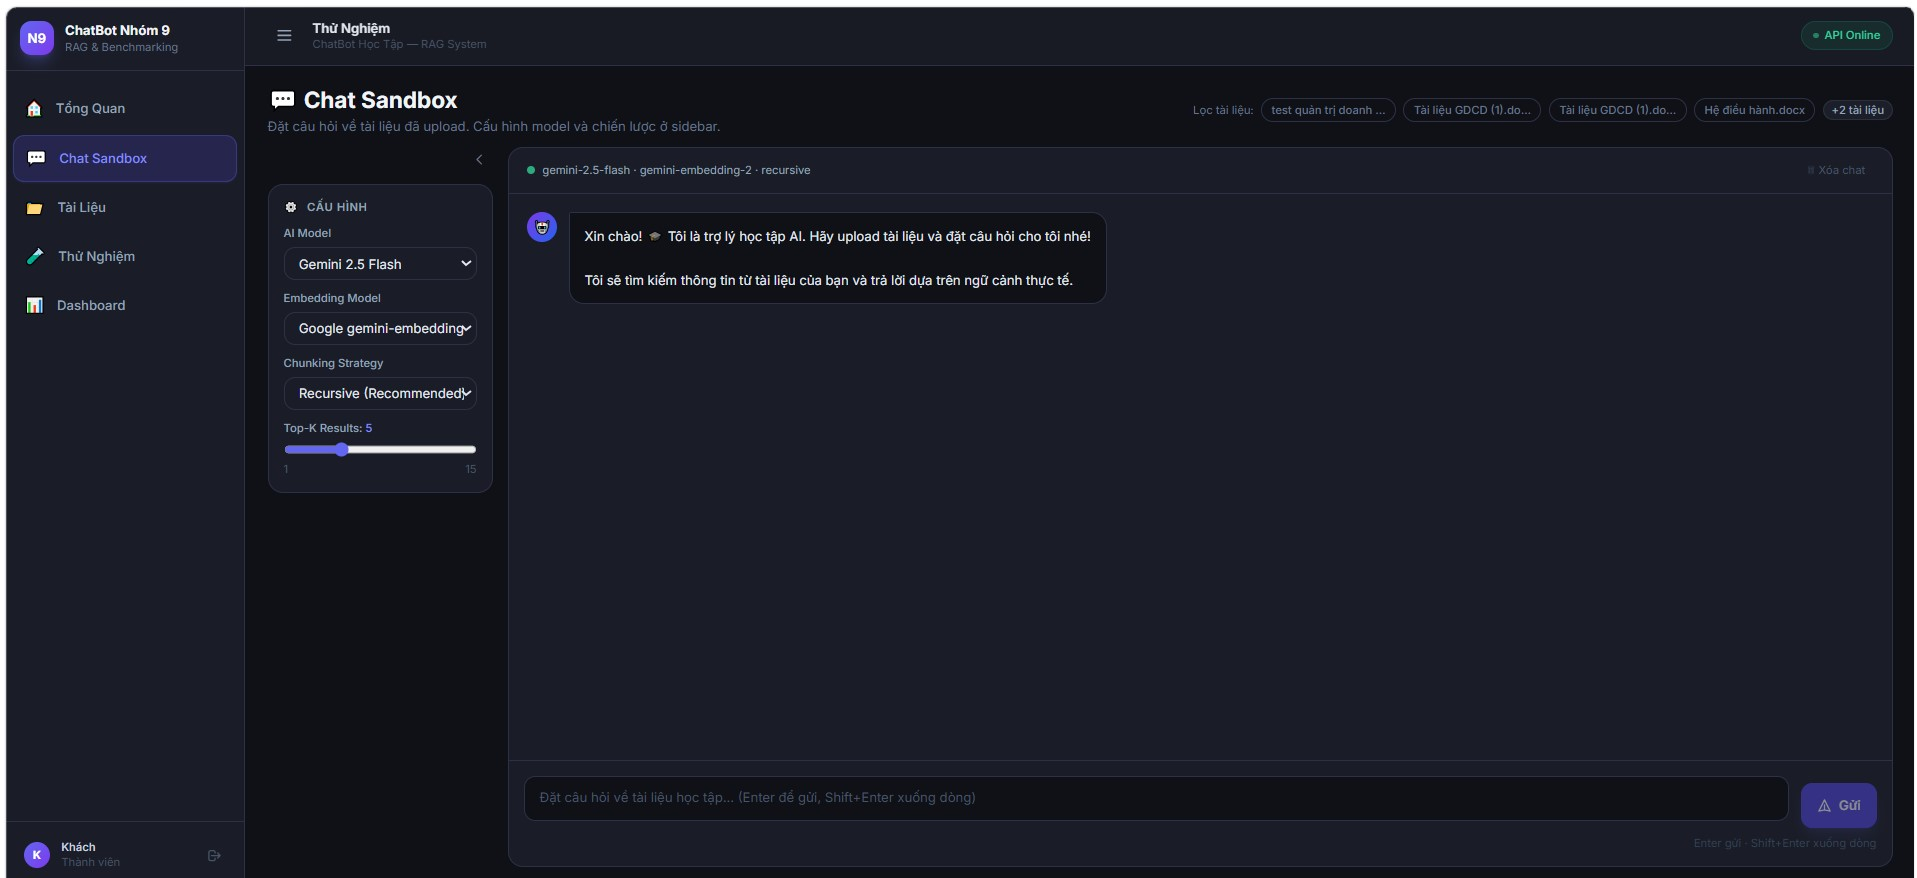
\includegraphics[width=\textwidth]{images/giao_dien_chat.jpg}
  \caption{Giao diện Chat Sandbox với bảng cấu hình RAG}
  \label{fig:ui-chat}
\end{figure}

\section{Kết luận Chương}

Chương này đã trình bày đầy đủ tài liệu thiết kế phần mềm (SWD) bao gồm: kiến trúc hệ thống 5 lớp, Package Diagram, ERD chi tiết với mô tả các bảng, Class Diagram với 11 lớp chính, State Machine Diagram (vòng đời tài liệu và phiên hội thoại), 3 Flowchart (RAG Pipeline, Ingestion Pipeline, Benchmark Pipeline), 3 Activity Diagram (Chat, Upload, Benchmark) và đặc tả Use Case chi tiết. Tất cả thiết kế được xây dựng nhất quán với SWR và tạo nền tảng kỹ thuật vững chắc cho giai đoạn triển khai và kiểm thử.
